\chapter{语义信息引导的视频目标跟踪算法研究}\label{chap:IGCF}

对于视频目标跟踪算法而言,判别表观学习具有极其重要的地位。在缺少目标类别先验的情况下,跟踪任意类别的目标通常需要在线进行目标前景与背景的判别信息学习。同时由于目标大小、形状、视角以及背景场景中光照、遮挡物、嘈杂干扰等都会随着时间发生剧烈变化。
基于传统相关滤波器(CF)的跟踪器通常仅依靠岭回归进行表观模型的建模,而不会感知目标在语义级别的实例信息。这种语义信息的缺乏可能导致跟踪漂移或跟踪器完全失效。为了解决这一问题,本章提出了实例引导的相关滤波器(instance guided correlation filter,IGCF),以提高跟踪的鲁棒性。具体来说,本章提出一个深层卷积神经网络(即 InstMask),旨在为目标生成实例级别的分割模板,该模板用于约束相关滤波器的学习。在实例级分割的基础上,本章进一步提出了一种自校正机制来缓解相关滤波跟踪器的漂移问题。在几个具有挑战性的基准测试数据库上进行的广泛实验验证了我们所提出的实例引导的相关滤波跟踪器的有效性。%,在单个 CPU 内核上的运行速度可达 5 帧每秒。

\section{引言}
目标跟踪是计算机视觉中的重要研究方向之一。给定视频起始帧中的目标位置,跟踪的目的是估计后续帧中目标的状态。尽管研究人员在该领域进行了长期的努力 \cite{Leang2018OnlineFO, Wang2019VisualOT, Zhang2018UsingFL},但在低功耗平台上仍难以实现可接受的跟踪精度和速度。另外,跟踪过程中的遮挡、照明变化、表观变化和快速运动等现象,使得目标跟踪算法难以在自动驾驶、机器人技术和增强现实等现实应用中难以进行部署和应用。

在过去的十年中,判别性相关滤波(discriminative correlation filter,DCF)跟踪器 \cite{MOSSE,Henriques2012ExploitingTC,Danelljan2014AdaptiveCA} 引起了研究人员的极大兴趣,此类跟踪器通过利用离散傅立叶变换以高效的方式利用了跟踪样本的所有空间偏移。然而,对于大多数 DCF 跟踪器而言,目标位置由一个矩形框描述。然而,对于形状不规则的目标,或具有环状结构的目标而言,矩形目标区域中将被掺杂大量的背景信息,这可能导致跟踪漂移和失效。此外,实例级别语义信息的缺失限制了 DCF 跟踪器的性能潜力。

基于 DCF 跟踪器的成功,许多研究 \cite{Danelljan2015LearningSR, Lukezic2017DiscriminativeCF} 已证明对目标进行空间约束可改善相关滤波器的表观建模。然而,大多数空间约束都是手工设计的,且未考虑有关目标的语义信息。尽管实例级语义分割 \cite{Pinheiro2015LearningTS, Zhang2019ProgressivelyDN}(旨在为图像中的每个像素分配语义标签)能够提取图像中的实例级语义信息,直接集成现有的实例分割方法以对相关滤波器的学习进行空间约束很难在跟踪精度和速度之间取得平衡。

\begin{figure}
\centering
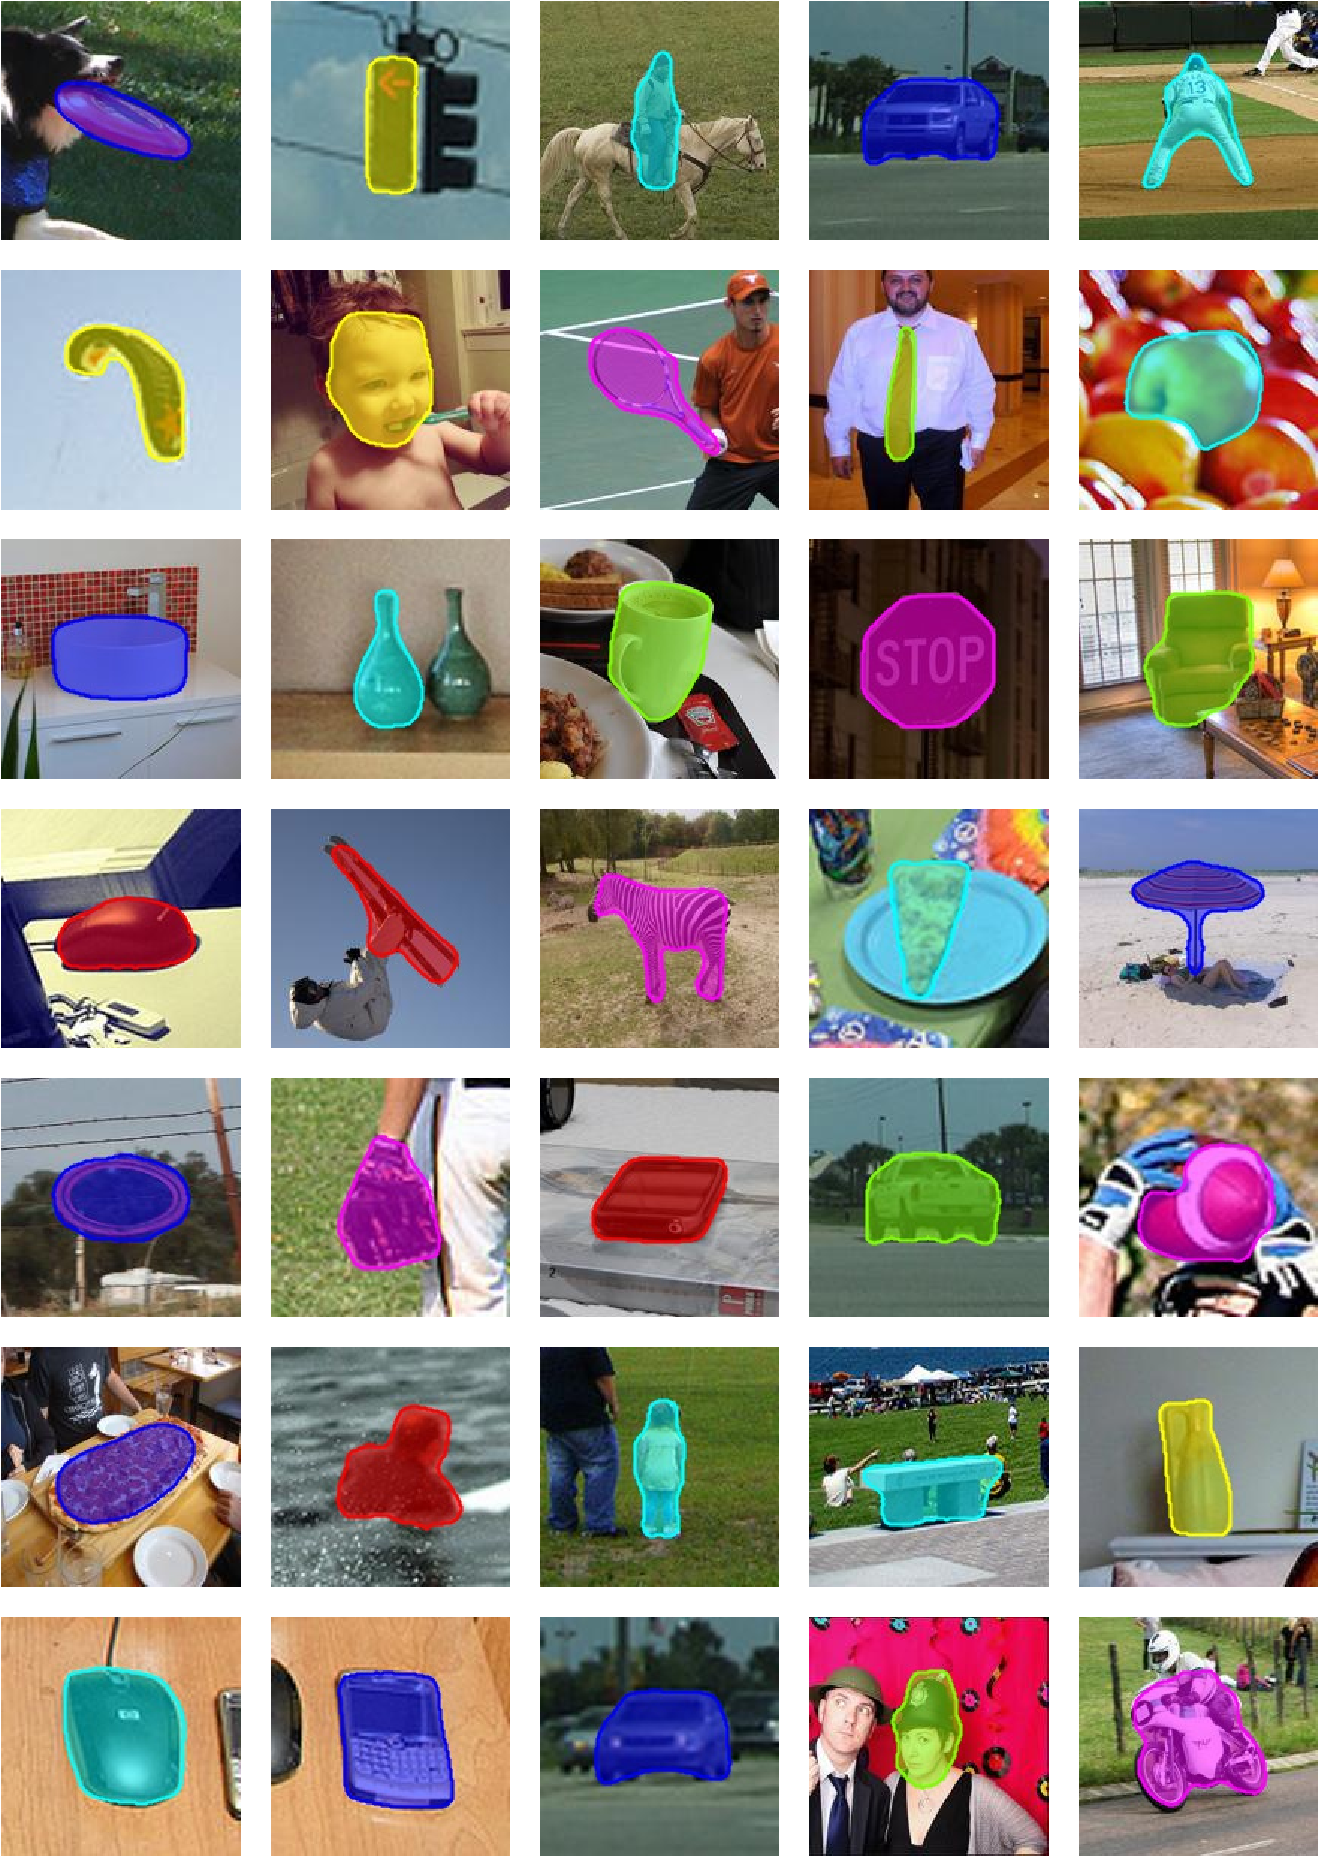
\includegraphics[width=1.0\textwidth]{Img/IGCF/coco.pdf}
\caption{InstMask 在 COCO2017 \cite{COCO} 验证集上的分割结果。}
\label{fig:IGCF_vis_coco}
\end{figure}

在本章中,我们提出了实例引导的相关滤波器(IGCF)来解决上述问题。具体而言,我们设计了一个深层卷积神经网络(即 InstMask),旨在准确生成目标实例级别的语义分割模板。我们利用 COCO2017 \cite{COCO} 对 InstMask 进行了离线的端到端训练(参见图 \ref{fig:IGCF_vis_coco})。实例级别的语义分割模板可以抑制背景噪声的干扰,从而显式约束相关滤波器的学习过程。
与常见的目标分割任务不同,我们设计了一种新的网络结构和训练方法,使得 InstMask 能够识别位于搜索图像中心附近的显著目标。值得注意的是,InstMask 可以识别任意类别的目标,而不仅限于识别训练集中出现的类别中的目标。此外,我们的网络中包括一个 $1 \times 1$ 卷积层,可以利用全局感受野从目标附近获取上下文信息,从而增加了分割的准确性。所提出的轻量级的分割网络可在单个 CPU 核心平台上以 5 FPS 的速度运行时,可在精度和速度之间取得平衡。

此外,我们注意到,为满足跟踪自适应性要求而在线更新的相关滤波器与满足鲁棒性要求的离线 InstMask 模块是独立且互补的。因此,两个组件的输出可以集成在一起,以进一步提高跟踪性能。具体而言,基于实例级别的分割,本章进一步提出了一种自校正机制来缓解相关滤波跟踪器的漂移问题。分割模板的几何中心用于校正相关滤波器的预测偏差。配备有 InstMask 模块的 IGCF 不仅可以精确地跟踪目标,还可以用于视频目标分割,这证明了我们算法的广泛应用。所提出的的跟踪框架 IGCF 的体系结构如图 \ref{fig:IGCF} 所示。

\begin{figure*}
    \centering
    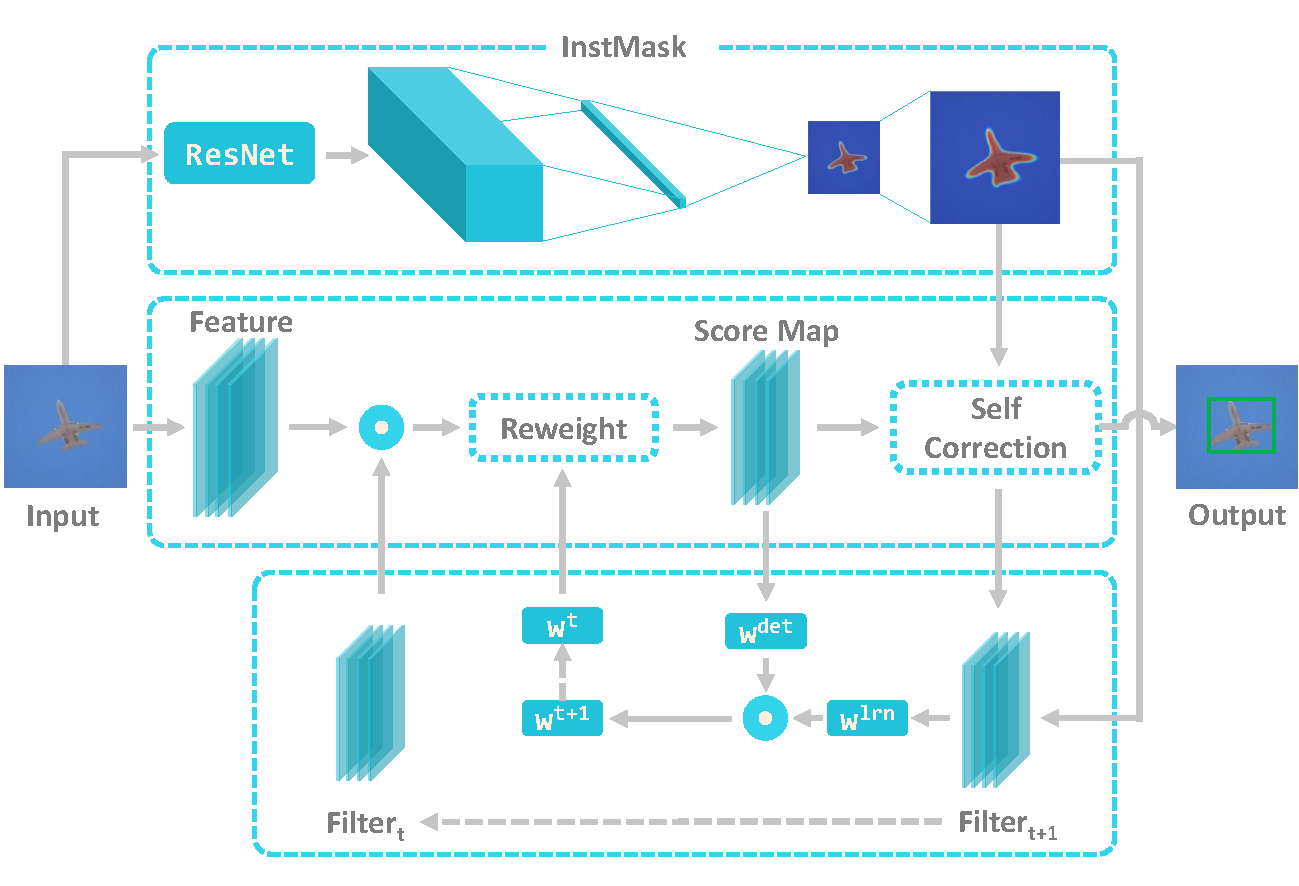
\includegraphics[width=1.0\textwidth]{Img/IGCF/instmask1.pdf}
    \caption{跟踪框架 IGCF 的结构。}
    \label{fig:IGCF}
\end{figure*}

我们在三个跟踪数据库上进行了全面的实验:VOT2015 \cite{Kristan2015TheVO}、VOT2016 \cite{Kristan2016TheVO} 和 GOT-10k \cite{GOT-10k}。我们的 IGCF 跟踪器在跟踪精度与跟踪速度方面取得了良好的平衡。最后,我们在视频目标分割数据集 DAVIS2016 \cite{Perazzi2016} 上进行了定性实验,以展示我们算法具有视频目标分割能力。

\section{相关工作}
几十年来,视频目标跟踪一直是主流的计算机视觉研究方向之一。视频目标跟踪的目的是在给定目标在第一帧中位置的情况下,确定目标在视频后续帧中的位置。

\subsection{基于相关滤波的跟踪器}
许多基于相关滤波的跟踪器旨在考虑部分遮挡、照明变化、背景混杂、运动模糊、视角变化等问题。

Bolme 等人 \cite{MOSSE} 提出基于平方误差最小输出和(MOSSE)滤波器的跟踪器。该跟踪器以每秒 669 帧的速度运行,可以抵抗光照变化、尺度变化,姿势变化和非刚性变形。
CSK 跟踪器 \cite{Henriques2012ExploitingTC} 通过采用图像子窗口的循环结构并使用快速傅里叶变换(FFT)快速合并来自所有子窗口的信息,对 MOSSE 跟踪器进行了改进。此外,文献 \cite{Henriques2012ExploitingTC} 表明,使用核技巧可以像在原始图像空间中一样高效地完成非线性空间中的分类。
在文献 \cite{Danelljan2014AdaptiveCA} 中,Danelljan 等人提出通过学习多维颜色属性的多通道滤波器来改进 CSK 跟踪器。为了避免由于颜色属性的高维度而导致的计算开销,作者提出了一种自适应维降技术,可以将原始的 11 维减少到只有 2 维。
后来,Henriques 等人 \cite{henriques2014high-speed} 为大量平移图像块提出了一种分析模型,并使用离散傅立叶变换将模型对角线化。该操作可以将存储和计算量减少几个数量级。

最近,许多研究 \cite{Danelljan2015LearningSR, Lukezic2017DiscriminativeCF} 已将空间约束引入到相关滤波器的学习中。在文献 \cite{Danelljan2015LearningSR} 中,作者提出了一种称为“空间正则化差异相关滤波器(SRDCF)”的跟踪器。SRDCF 在学习过程中引入了空间正则化组件,以根据相关滤波器系数的空间位置对它们进行惩罚。
此外,文献 \cite{Lukezic2017DiscriminativeCF} 提出的 CSR-DCF 滤波器将通道和空间可靠性组件引入了相关滤波跟踪器,并为它们在滤波器更新和跟踪过程中的有效无缝集成提供了学习算法。空间可靠性组件将滤波器用于适应目标的空间位置。通道可靠性组件根据特征的通道信息生成特征加权系数。CSR-DCF 跟踪器具有较大的搜索区域,可以有效跟踪非矩形目标。空间可靠性组件与 Staple \cite{Bertinetto2016StapleC} 跟踪器中使用的颜色分布具有一些相似之处,该工作解决了相关滤波器的模板模型和逐像素颜色分布模型的两个独立的岭回归问题。
为了处理目标的尺度变化,Li 等人 \cite{Li2014ASA} 提出的方法以不同的尺度对目标进行采样,并将采样调整为固定大小,以便与每帧的模型相匹配。此方法还采用了多特征集成方案,该方案使用原始像素、梯度直方图 \cite{Forsyth2014ObjectDW} 和颜色名称特征 \cite{Weijer2009LearningCN} 来进一步增强跟踪器的性能。这些基于 DCF 的跟踪器的主要缺点是缺乏对目标的高级语义信息的感知。

\subsection{基于卷积神经网络的跟踪器}
在过去的几年中,深度学习 \cite{Goodfellow2015DeepL} 在许多研究领域都取得了显著成功,尤其是在计算机视觉 \cite{Matiz2019InductiveCP, Zhu2019RotatedCR, Xiao2019DenseSE},语音识别 \cite{Kim2016JointCB, Liu2019AttentionGD} 和自然语言处理 \cite{Vinyals2014GrammarAA, Yousfi2017ContributionOR} 等领域。一些跟踪器已经证明了深度学习的性能优势。

大多数基于 DCF 的跟踪器仅限于单分辨率特征图,从而极大地限制了其潜力。为了解决此问题,CCOT 跟踪器 \cite{CCOT} 学习连续卷积滤波器以融合以不同分辨率获得的特征图。这将为目标生成连续域置信度图。除了多分辨率融合之外,连续域学习公式还可以实现精确的亚像素定位。
ECO 跟踪器 \cite{Danelljan2017ECOEC} 在 DCF 公式中引入分解卷积算子训练样本分布的紧凑生成模型,并采用保守的模型更新策略。ECO 使用了 CNN 特征,同时减轻了计算开销。CF2 跟踪器 \cite{Ma2015HierarchicalCF} 自适应地学习每个卷积层上的相关滤波器,以对目标表观进行编码,并使用每一层的相关响应来推断目标位置。

在文献 \cite{GOTURN} 中,Held 等人提出了一种离线训练的神经网络来进行跟踪目标,使用简单的前馈网络,而无需在线训练。该网络可感知目标运动与表观之间的一般关系,并可用于跟踪未出现在训练集中的新目标。
最近,一系列跟踪器(例如 SiamFC \cite{SiamFC}、SiamRPN \cite{SiamRPN}、DasiamRPN \cite{zhu2018distractor} 和 SiamMask \cite{Wang2018SiamMask})使用孪生网络来学习搜索图像和模板图像之间的相似性。它们在跟踪速度和准确性之间取得了良好的平衡。SiamMask 是在一个端到端学习框架中同时执行跟踪和分割的首次尝试。尽管在准确性和鲁棒性方面都具有良好的性能,但是上述大多数跟踪器都具有很高的特征提取计算开销,因此不适合于低功耗平台。例如,SiamMask 算法在 Intel E5-2620 CPU 平台上的运行速度仅为 1 帧每秒。

也有一些工作致力于使用自校正机制来减轻跟踪漂移,从而提高跟踪的鲁棒性。例如,在文献 \cite{fan2018parallel} 中,跟踪框架由两个组件(跟踪器和验证器)组成,它们在两个单独的线程上并行工作。跟踪器提供实时跟踪推断,并有望在大多数情况下表现良好。相反,验证者检查跟踪结果并在需要时更正跟踪器。

\section{实例引导的相关滤波器}

\begin{algorithm}[t]
  \caption{IGCF 跟踪算法} 
  \begin{algorithmic}
    \Require 图像 $I_t$,目标在上一帧中的位置 $p_{t-1}$、尺度 $s_{t-1}$、滤波器 $h_{t-1}$,通道可靠性 $w_{t-1}$。
    \Ensure 位置 $p_t$,尺度 $s_t$ 和更新后的模型。
  \Statex
  \State \textbf{定位:}
  \begin{enumerate}[leftmargin=0pt,itemindent=1.5em]
    \item $p_t$:$h_{t-1}$ 和从位置 $p_{t-1}$ 提取的图像块的特征 $f_{t}$ 进行相关后的最大响应的位置,由信道可靠性得分加权 $w_{t-1}$(等式 \ref{eq:dcf})。
    \item 估计分割模板 $m$(第 \ref{sec:InstMask} 节)。
    \item 使用 $m$ 校正 $p_t$ (第 \ref{sec:cog} 节)。
    \item 使用位置 $p_t$ 估计新的尺度 $s_ t$ (参考 \cite{Danelljan2014AccurateSE})。
    \item 使用等式 \ref{eq:det},根据逐通道响应,估计检测可靠性 $\tilde{w}^{(det)}$。
  \end{enumerate}
  \State \textbf{更新:}
  \begin{enumerate}[leftmargin=0pt,itemindent=1.5em]
    \item 使用等式 \ref{eq:h1}至等式 \ref{eq:h3},根据 $m$ 估计新滤波器 $\tilde{h}$。
    \item 使用等式 \ref{eq:lrn},根据 $h$ 估计学习通道可靠性 $\tilde{w}^{(lrn)}$。
    \item 使用等式 \ref{eq:c} 计算通道可靠性 $\tilde{w}$。
    \item 使用等式 \ref{eq:update1} 和等式 \ref{eq:update2} 更新滤波器 $h_t$ 和通道可靠性 $w_t$。
  \end{enumerate}
\end{algorithmic}
\end{algorithm}

\subsection{相关滤波跟踪器}
相关滤波跟踪器 \cite{Danelljan2014AccurateSE, henriques2014high-speed, Li2014ASA} 已得到广泛研究和使用。具体来说,考虑目标的表观特征:$f=\{f_d\}_{d=1:N_c}$ ,其中 $N_c$ 是目标特征的通道数。DCF 跟踪器的目标是训练滤波器 $h=\{h_d\}_{d=1:N_c}$,以使特征和滤波器之间的相关性响应 $\tilde{g}$ 拟合所需输出 $g$ ,通常是一个以目标位置为中心的二维高斯函数: 
\begin{equation} \label{eq:dcf}
\tilde{g}=\sum_{d=1}^{N_c}f_d \star h_d \cdot w_d,
\end{equation}
其中 $\star$ 表示循环相关运算符,通道权重 $w = \{w_d\}_{d=1:N_c}$ 是基于每个特征通道 \cite{Lukezic2017DiscriminativeCF} 判别力的缩放因子。
响应图的峰值位置是目标在当前帧中的估计位置。
最佳相关滤波器 $h$ 通过最小化如下公式来估算:
\begin{equation}
\varepsilon(h) = \sum_{d=1}^{N_c}||f_d \star h_d - g||^2+\lambda||h_d||^2.
\end{equation}

最近,许多研究 \cite{Danelljan2015LearningSR, Lukezic2017DiscriminativeCF} 已经证明,为目标施加空间约束可通过减少背景干扰来改善相关滤波器的学习。如文献 \cite{Lukezic2017DiscriminativeCF} 中所述,图像补丁的分割模板是一个元素为 1 或 0 的空间掩码,用于指示像素属于目标还是属于背景。在滤波器的训练过程中,滤波器 $h$ 受模板 $m$ 约束:$h \equiv m \odot h$,其中 $\odot$ 表示逐元素乘积。该约束可使滤波器适应目标中适合跟踪的前景信息,从而可使用较大的训练区域来捕获更多上下文信息,并克服了矩形框的局限性。

\subsection{InstMask}
\label{sec:InstMask}

\begin{table}[t!]
\centering
\caption{InstMask 的网络结构设计。}
\begin{tabular}{ccc}
\toprule
层数 & 输出尺寸 & 卷积操作 \\\midrule
输入图像 & $160 \times 160 \times 3$ &  -\\\midrule
\multirow{2}*{主干块} & $80 \times 80 \times 64$ &  $ 7 \times 7 \text{ 卷积} $\\
~ & $40 \times 40 \times 64$ &  $ 2 \times 2 \text{ 最大池化} $\\\midrule
残差块(1)& $40 \times 40 \times 256$ &  $ \left [ \begin{array}{l} 1 \times 1 \text{ 卷积} \\ 3 \times 3 \text{ 卷积} \\ 1 \times 1 \text{ 卷积} \end{array} \right ] \times 3 $\\\midrule
残差块(2)& $20 \times 20 \times 512$ &  $ \left [ \begin{array}{l} 1 \times 1 \text{ 卷积} \\ 3 \times 3 \text{ 卷积} \\ 1 \times 1 \text{ 卷积} \end{array} \right ] \times 4 $\\\midrule
残差块(3)& $10 \times 10 \times 1024$ &  $ \left [ \begin{array}{l} 1 \times 1 \text{ 卷积} \\ 3 \times 3 \text{ 卷积} \\ 1 \times 1 \text{ 卷积} \end{array} \right ] \times 6 $\\\midrule
\multirow{5}*{解码器} & $10 \times 10 \times 128$ &  $ 1 \times 1 \text{ 卷积} $\\
~ & $1 \times 1 \times 512$ &  $ 10 \times 10 \text{ 卷积} $\\
~ & $1 \times 1 \times 3136$ &  $ 1 \times 1 \text{ 卷积} $\\
~ & $56 \times 56$ & 调整特征尺寸 \\
~ & $160 \times 160$ & 上采样 \\\bottomrule
\end{tabular}
\label{tab:InstMask}
\end{table}

\begin{figure*}[t]
    \centering
    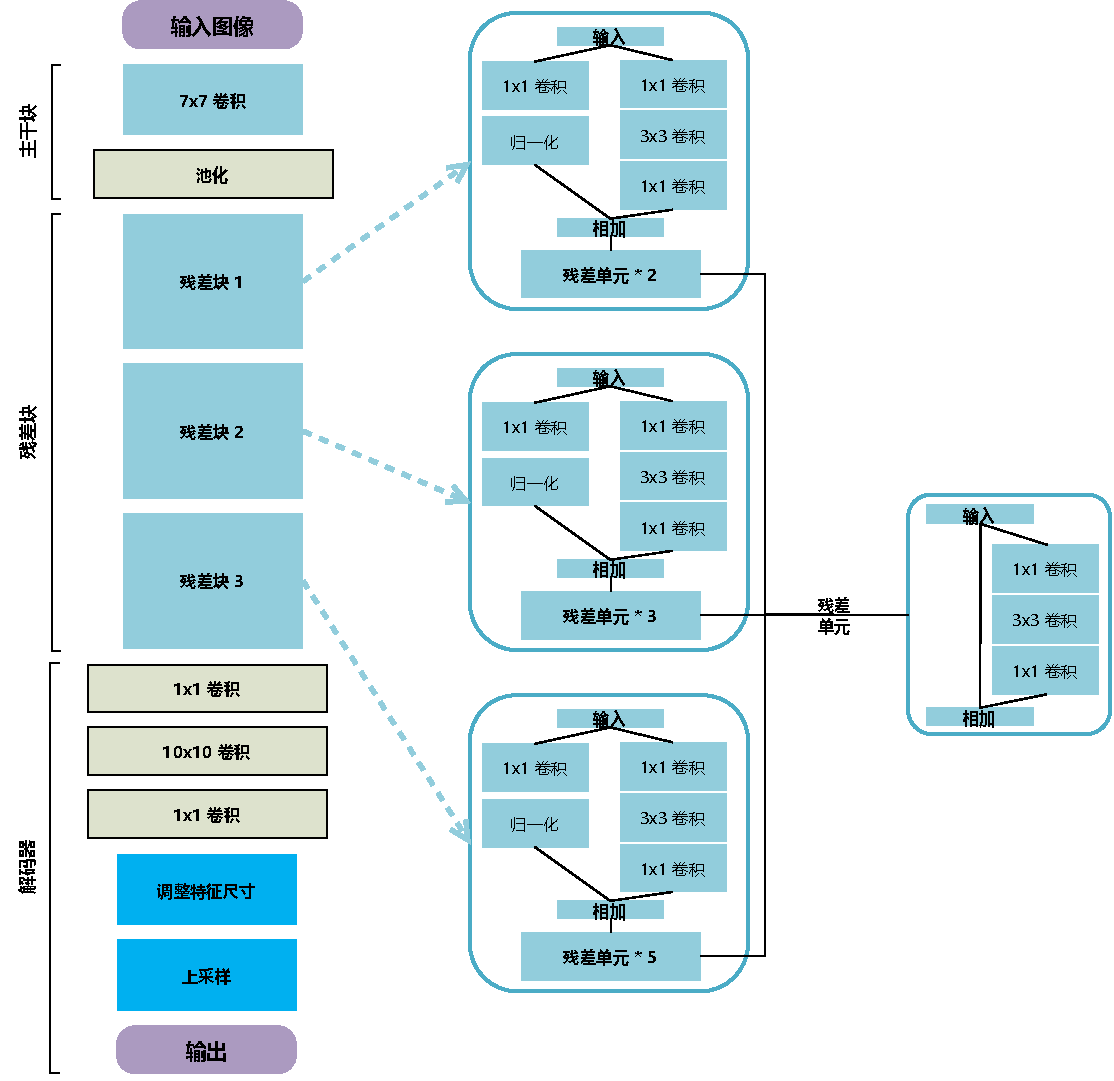
\includegraphics[width=1.0\textwidth]{Img/IGCF/net.pdf}
    \caption{InstMask 的网络结构。}
    \label{fig:IGCF_net}
\end{figure*}

在本章中,我们使用被跟踪目标的分割模板来约束相关滤波器的学习。出于效率和性能方面的考虑,理想的分割方法应具有三个关键特点:

\begin{itemize}
\item 与跟踪过程的无缝集成;
\item 足够简单以适应跟踪的速度要求;
\item 设计的分割算法应尽可能准确地预测目标的轮廓。
\end{itemize}

以前大多数用于生成空间约束的方法都依赖于手工设计的规则或低级图像特征(例如颜色直方图)。
在本章中,我们提出了 InstMask 网络,该网络为目标生成准确的实例分割模板。我们使用数据驱动的方法对 InstMask 进行离线地端到端训练,以从分割训练集(例如 COCO2017 \cite{COCO})中学习语义信息。实例级别的语义分割模板可以通过抑制背景信息来约束相关滤波器的学习。在实例级分割的基础上,我们进一步提出了一种自校正机制来减轻相关滤波跟踪器的漂移问题。与传统的相关滤波跟踪方法相比,此方法可显着提高目标跟踪精度。
与以前的生成分割模板的方法不同,我们不依赖于边缘、超像素或其他形式的低级信息。相反,我们模型的核心是卷积神经网络。通过利用在 ImageNet \cite{ImageNet} 上训练的强大卷积特征表示并拟合 COCO 中的大量分割训练数据,我们能够为目标生成准确的语义分割模板,以限制相关跟踪器的学习。
值得注意的是,将现有的实例分割方法进行集成到跟踪器中从而为相关滤波器的学习提供空间约束是次优的。通用跟踪算法通常具有复杂的网络结构,因此很难在跟踪精度和速度之间取得平衡。相比之下,本文提出的分割网络是专为跟踪而设计的,可在 CPU 上以 5 FPS 的速度运行。

当在第 $i$ 帧中跟踪时,需要获得第帧 $i$ 中目标的分割模板以约束相关滤波器的学习。
假定第 $i$ 帧中的目标位置在第 $i-1$ 帧中的目标位置附近,因此 InstMask 的输入始终是前一帧以目标位置为中心的小图像区域。
该设计具有以下优点:

\begin{itemize}
\item 由于输入数据的强一致性,网络可以使用较少的参数获得准确的分割结果。
\item 由于网络参数较少且图像补丁较小,因此推理时间短。
\item 在目标的先前位置附近进行搜索可以避免位于背景中近似物体的不利影响。
\end{itemize}

在训练期间,训练集中的每个样本 $k$ 包含(1)RGB 图像补丁 $x_k$,目标位于图像补丁中心附近,(2)图像补丁所对应的二进制分割模板 $m_{k}$。
接下来,我们描述体系结构和训练过程。

\textbf{体系结构} 表 \ref{tab:InstMask} 和图 \ref{fig:IGCF_net} 中显示了网络体系结构。InstMask 的主干是基于 ResNet50 \cite{He2016DeepRL} 构建的,它由一个主干块和三个残差块组成。
InstMask 的输入是一个 160$\times$160$\times$3 图像补丁。它被发送到主干块,生成尺寸为 40$\times$40$\times$64 的特征图。然后将特征图依次送入 3 个残差块,分别生成大小为 40$\times$40$\times$256,20$\times$20$\times$512,10$\times$10$\times$1024 的特征图。随后,将获得的特征图送入三个卷积层以生成长度为 3136 的向量,该向量具有全局感受野,能够感知有关目标的所有上下文信息。最后,将此向量尺寸调整为 56$\times$56,以获得最终的分割模板。InstMask 是一个轻量级的网络,可以在具有 Intel E5-2620 CPU 内核的平台上以 5 FPS 运行,能够较好地平衡跟踪准确性和速度,使跟踪器在包括自动驾驶、机器人技术和增强现实等实际应用中进行部署成为可能。

\textbf{训练} 在训练期间,将空间分辨率为 56$\times$56 的模板上采样至原始图像大小 160$\times$160。令 $l$ 表示大小为 $w \times h$ 的逐个像素的真实模板。损失计算如下:
\begin{equation}
L = \frac{1}{wh} \sum_{xy}{log(1+e^{-l_{x,y}P_{x,y}})},
\end{equation}
其中 $l_{x,y} \in \{ \pm 1 \}$ 是与对象模板的像素 $(x,y)$ 对应的标签,而 $P_{x,y}$ 是 InstMask 的预测在位置 $(x,y)$。

我们采用 COCO2017 \cite{COCO} 实例分割数据集对 InstMask 进行训练。
与许多只能预测训练集中出现的类别的分割网络不同,提出的 InstMask 在训练过程中会忽略类别信息,并作为与类别无关的分割网络工作。实际上,InstMask 能够在搜索区域中检测到显著目标。尽管 InstMask 使用仅有 80 个类别的 COCO 数据集 \cite{COCO} 进行训练,但是网络能够对训练集中未出现的目标类别进行分割,如图 \ref{fig:IGSC} 所示。
在训练期间,输入图像大小设置为 160$\times$160,目标位于图像的中心,大小为 112$\times$112。为了增强网络的通用性,我们执行数据增强。具体来说,我们考虑平移($\pm$16 像素),缩放变形( $2^{\pm 1/4}$)以及水平翻转。
InstMask 离线训练。在跟踪过程中,InstMask 仅执行前向传播过程,而不会进行梯度的后向传播。这不仅可以防止漂移,还可以满足实时跟踪要求。

尽管我们的模型与 CSRDCF \cite{Lukezic2017DiscriminativeCF} 具有高度的相似性,但实现原理却大不相同。
在 CSRDCF \cite{Lukezic2017DiscriminativeCF} 中,使用目标和背景的颜色直方图生成分割模板。这种启发式方法具有几个缺点:

\begin{itemize}
\item 由于仅使用低级像素信息,因此难以准确地分割目标。
\item 为了适应目标的表观变化,在跟踪过程中会不断更新直方图模型,这很容易导致跟踪器漂移。
\end{itemize}

相反,InstMask 不会在线更新参数。这提高了计算效率,同时避免了跟踪器的漂移。此外,由于使用语义级别而不是像素级别的信息进行分割,因此跟踪结果更加准确。

\subsection{实例引导的自纠正组件} \label{sec:cog}

\begin{figure*}[t]
    \centering
    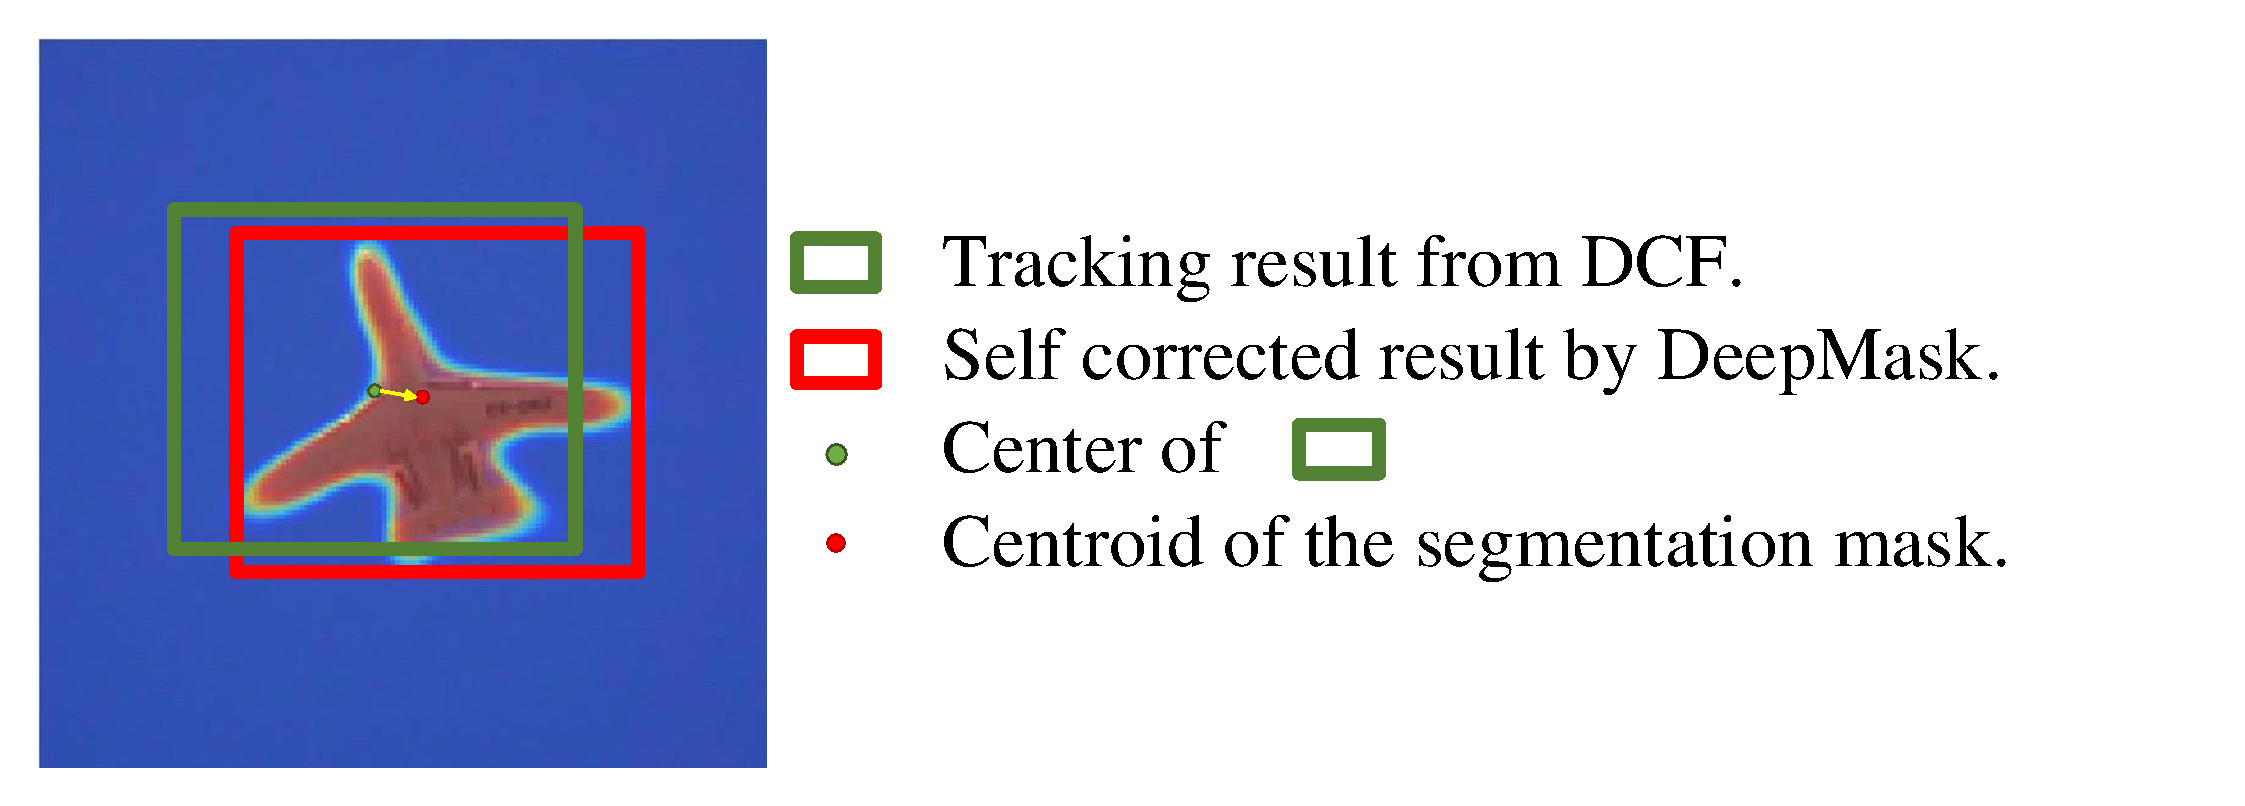
\includegraphics[width=0.7\textwidth]{Img/IGCF/cog_arch.pdf}
    \caption{实例引导的自纠正原理图。}
    \label{fig:cog}
\end{figure*}

InstMask 允许学习更好的滤波器,并有助于纠正不良的跟踪结果。
在 DCF 模块中,滤波器 $h$ 和特征 $f$ 之间的最大相关位置被认为是当前帧中的目标位置。但是,由于在线更新,相关滤波器很容易漂移。
InstMask 的结果是根据从 COCO 数据集中获取的网络参数生成的。但是,由于 InstMask 不会在线更新,因此我们不能仅依靠目标的语义分割模板来产生最终的跟踪结果。
为了利用两个结果的优点并克服它们的缺点,我们提出了实例引导的自纠正(instance guided self-correction,IGSC)组件。IGSC 结合了实例分割和相关滤波结果,以提高跟踪的鲁棒形。具体来说,使用硬阈值 $b$ 根据 $P\in [0, 1]$ 生成模板 $m$:
\begin{equation}
m_{x,y} = \left\{ \begin{array}{ll}
 1 & \textrm{if $P_{x,y} > b$}\\
 0 & \textrm{if $P_{x,y} \le b$}
 \end{array} \right.
\end{equation}
$P$ 是从 InstMask 生成的概率图。元素 $P_{x,y}$ 是像素 $(x,y)$ 属于目标的概率。
然后从 $m$ 获得目标位置:
\begin{equation}
c_{m} = Centroid(m),
\end{equation}
其中 $Centroid(\mathord{\cdot})$ 可以计算区域的几何中心。
将 $p$ 表示为校正后的目标位置。
自校正过程可以描述如下:
\begin{equation}
p = \left\{ \begin{array}{ll}
 c_{m} & \textrm{if $||c_{m}-c_{dcf}||_2^2 < \beta$}\\
 c_{dcf} + \alpha \cdot (c_{m}-c_{dcf}) & \textrm{其他}
 \end{array} \right.,
\end{equation}
其中 $c_{dcf}$ 是 DCF 预测的位置,$\alpha$ 是控制自校正强度的超参数,而 $\beta$ 是 $c_{m}$ 和 $c_{dcf}$ 之间距离的阈值。
由于分割结果的鲁棒性,当 DCF 结果显示不稳定漂移时,跟踪器可以自行校正。图 \ref{fig:IGSC} 中显示了提出的实例指导的自校正组件的有效性。

\begin{figure}
\centering
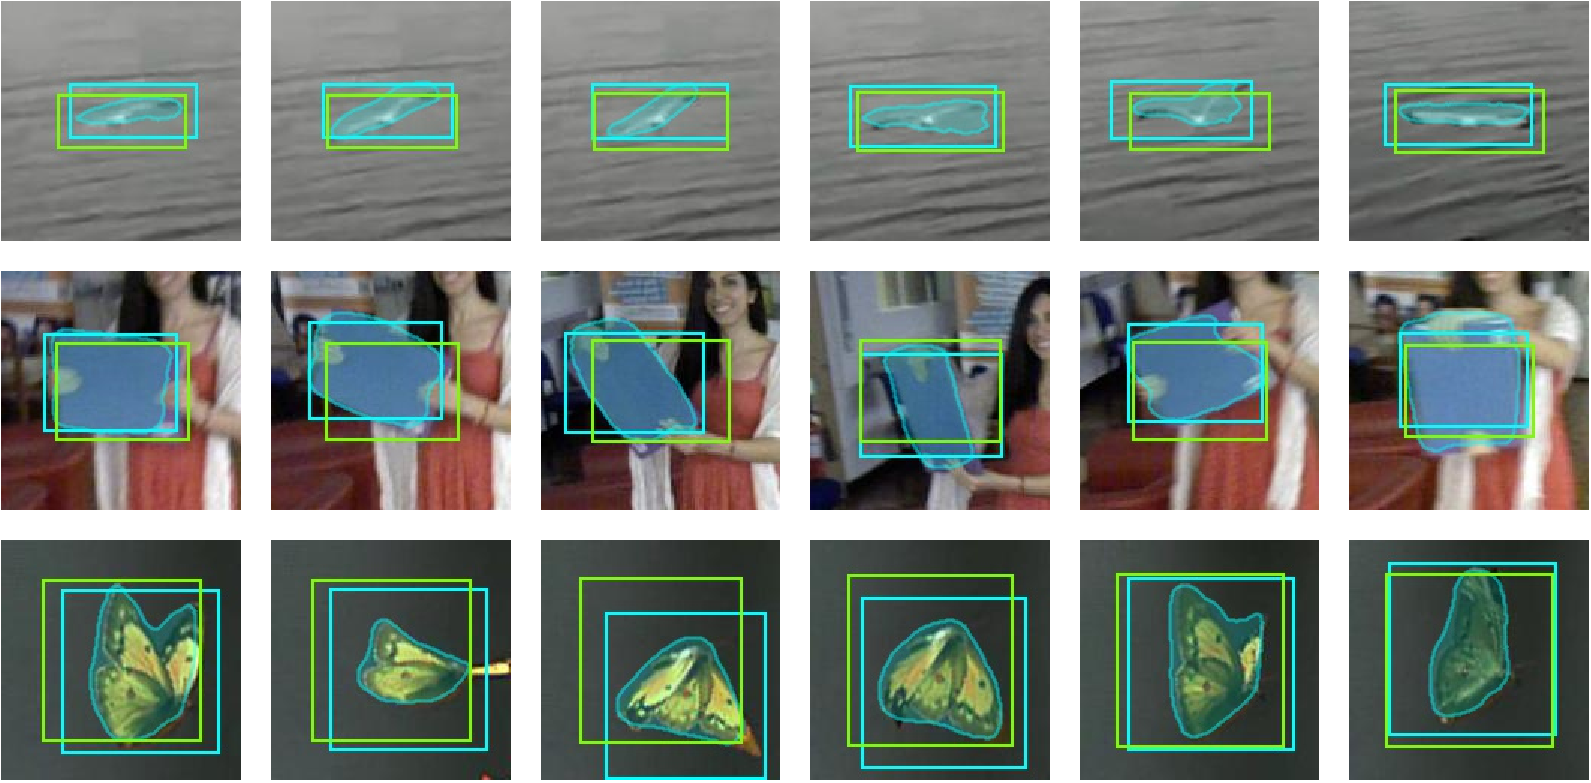
\includegraphics[width=1.0\textwidth]{Img/IGCF/cog.pdf}
\caption{实例指导(自我校正)组件之前(绿色)和之后(蓝色)的跟踪结果。}
\label{fig:IGSC}
\end{figure}

\subsection{跟踪过程}
跟踪过程包括两个阶段:目标定位和模型更新。
在定位阶段,从位置 $p_{t-1}$ 提取图像补丁特征 $f$,与滤波器 $h_{t-1}$ 进行相关计算,并根据通道依赖性得分 $w$ 加权,目标位置 $p_t$ 是相关结果的最大位置(等式 \ref{eq:dcf})。
使用本章提出的 InstMask 网络估计分割模板 $m$ (第 \ref{sec:InstMask} 节)。
分割模板的质心用于校正相关滤波器的预测偏差 (第 \ref{sec:cog} 节)。
然后新的尺度 $s_t$ 由尺度空间相关滤波器估计(参见 \cite{Danelljan2014AccurateSE})。
通道检测可靠性 $\tilde{w}^{(det)}$ 估算如下 \cite{Lukezic2017DiscriminativeCF}:
\begin{equation} \label{eq:det}
\tilde w_d^{(det)} = max(1 - \rho_d^{max2} / \rho_d^{max1}, 0.5),
\end{equation}
$\tilde w_d^{(det)}$ 用于稍后计算 $w$ (等式 \ref{eq:c})。$\rho_d^{max2}$ 和 $\rho_d^{max1}$ 分别是通道 $d$ 的相关响应中第二高/第一高的非相邻峰值。

在模型更新阶段,新的滤波器 $\tilde{h}$ 使用模板 $m$ 进行估计。我们使用 \cite{Lukezic2017DiscriminativeCF} 中提出的迭代方法来有效地解决滤波器。令 $l$ 为拉格朗日乘数,$\mu > 0$,$h_m=m \odot h$,$\hat{h}^0 = h_{t-1}$ 和 $\hat{l}^0 = 0$。在每次迭代中,都按照 \cite{Lukezic2017DiscriminativeCF} 中的顺序依次解决以下子问题:
\begin{equation} \label{eq:h1}
\hat{h}_c^{i+1} = \frac{\hat{f} \odot \bar{\hat{g}} +(\mu^i \hat{h}_m^i - \hat{l}^i)}{\bar{\hat{f}} \odot \hat f + \mu^i}
\end{equation}
\begin{equation}
h^{i+1} = \frac{m \odot \mathcal{F}^{-1}[\hat{l}^i + \mu^i\hat{h}_c^{i+1}]}{\frac{\lambda}{2D} + \mu^i}
\end{equation}
\begin{equation} \label{eq:h3}
\hat{l}^{i+1} = \hat{l}^i + \mu(\hat{h}_c^{i+1} - \hat{h}^{i+1})
\end{equation}
然后计算通道可靠性 $\tilde w_d$ \cite{Lukezic2017DiscriminativeCF} 如下,其中包括通道学习可靠性 $\tilde w_d^{(lrn)}$ 和通道检测可靠性 $\tilde w_d^{(det)}$:
\begin{equation} \label{eq:c}
\tilde w_d = \tilde w_d^{(lrn)} \cdot \tilde w_d^{(det)},
\end{equation}
其中 $\tilde{w}^{(lrn)}$ 表示学习的通道滤波器的最大响应值:
\begin{equation} \label{eq:lrn}
\tilde{w}_d^{lrn} = max(f_d * h_d).
\end{equation}
最后,滤波器和通道可靠性在线更新:\begin{equation} \label{eq:update1}
h_t = (1 - \eta)h_{t-1} + \eta \tilde{h}
\end{equation}
\begin{equation} \label{eq:update2}
w_t = (1-\eta)w_{t-1} + \eta \tilde{w},
\end{equation}
其中 $\eta$ 是用于控制模型更新速度的学习率。

\section{实验评估与分析}

\begin{figure}[t]
    \centering
    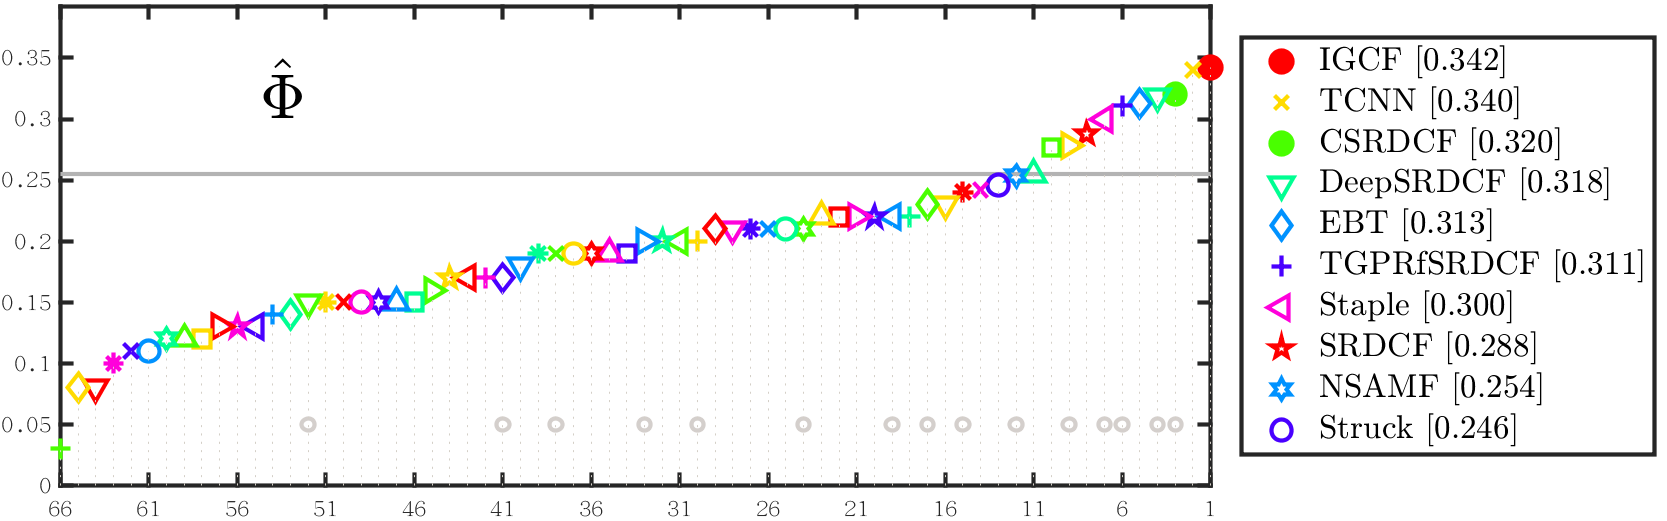
\includegraphics[width=1.0\textwidth]{Img/IGCF/vot/eao_rank_vot2015.png}
    \caption{VOT2015 的预期平均重叠(EAO)图 \cite{Kristan2015TheVO}.}
    \label{fig:vot15}
\end{figure}

\subsection{实验设置}
\textbf{网络架构设计}:本章所提出的用于对相关滤波跟踪器提供语义引导信息的分割网络 InstMask 主要由两个子网络构成,分别是用于特征提取的主干网络和用于生成分割模板的解码网络。它们的网络结果如表 \ref{tab:InstMask} 所示,网络主干包含三个残差块,可以快速将搜索图像区域图像的分辨率下降到较低尺度,以提升计算效率。

\textbf{训练数据}:为了提高分割结果的泛化能力,同时避免在稀缺的跟踪数据上过度拟合,InstMask 的离线训练过程在大规模图像分割数据集 COCO2017 \cite{COCO} 的训练数据集中训练网络参数。该数据集以场景理解为目的,主要从复杂的日常场景中截取,图像中的目标通过精确的分割进行位置的标定,包含超过 33 万张图片和 80 个类别。该数据集被广泛使用在最近提出的图像分割算法 \cite{He2018MaskR} 训练中。

\textbf{优化器参数设定}:本章使用动量为 0.9 的随机梯度下降(stochastic gradient descent,SGD)优化器从随机初始化的网络参数开始训练,并将权值衰减参数设置为 0.00005。学习率从 $10^{-2}$ 指数衰减到 $10^{-4}$。该模型经过 50 个迭代周期的训练,每个批量大小为 32 个样本。

本章所提出的用于对相关滤波跟踪器提供语义引导信息的分割网络 InstMask 使用 MatConvNet \cite{MatConvNet} 在 MATLAB 平台上实现,所有实验在装配有 Intel(R) Xeon(R) CPU E5-2630 v4 @ 2.20GHz 和 NVIDIA TITAN 1080Ti GPU 的工作站上执行。

我们在三个具有挑战性的目标跟踪数据集上对提出的跟踪器 IGCF 进行了全面评估:VOT2015 \cite{Kristan2015TheVO},VOT2016 \cite{Kristan2016TheVO} 和 GOT-10k \cite{GOT-10k}。请注意,用于训练 InstMask 组件的视频与评估数据集之间没有重叠。最后,我们对视频目标分割数据集 DAVIS \cite{Perazzi2016} 进行了定性实验。

\begin{figure}[t]
    \centering
    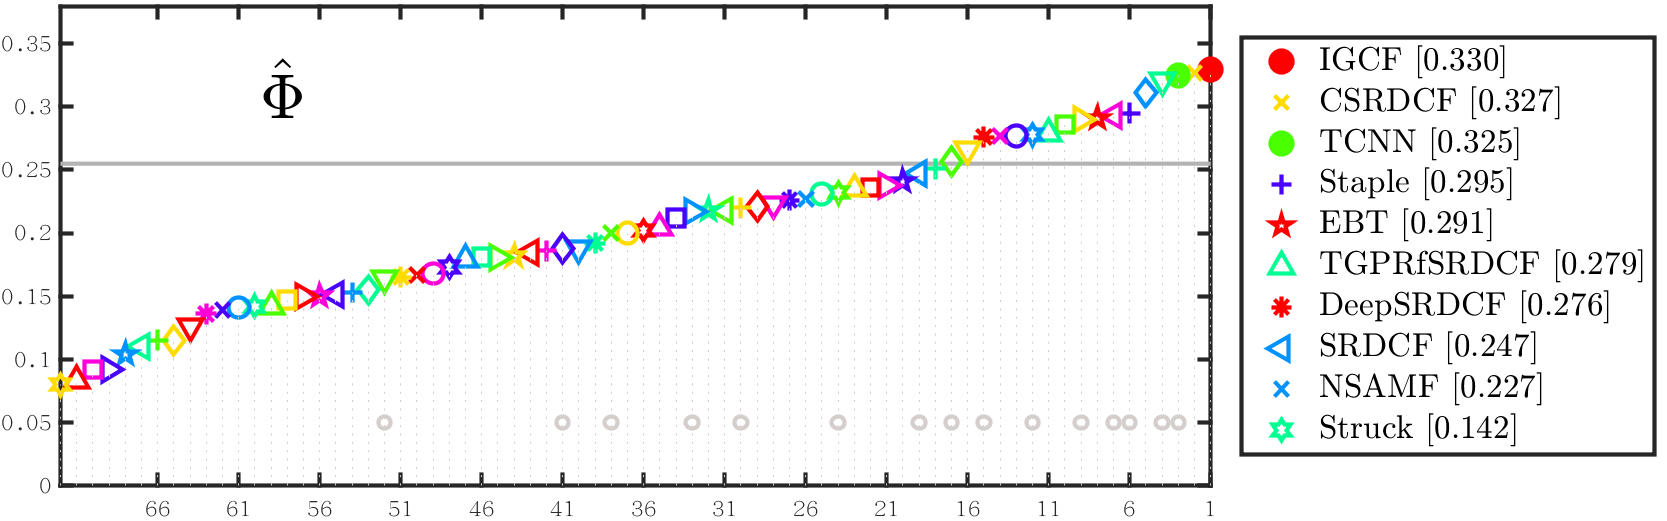
\includegraphics[width=1.0\textwidth]{Img/IGCF/vot/eao_rank_vot2016.png}
    \caption{VOT2016 的预期平均重叠(EAO)图 \cite{Kristan2016TheVO}。}
    \label{fig:vot16}
\end{figure}

\subsection{对 VOT2015 的评估}
在本节中,将使用视觉目标跟踪工具包的最新版本进行实验对比。该工具包采用基于目标重置的跟踪性能评估方法。评估算法一旦检测到跟踪器发生错误跟踪(即跟踪器预测和真实目标标签的重叠率为 0),就会在错误帧后的第五帧重新初始化跟踪器。
%测评性能使用期望平均重叠率(EAO)来度量排序,EAO 指标同时定量反映算法的鲁棒性和准确性。
VOT2015 \cite{Kristan2015TheVO} 跟踪数据集包含 60 个具有挑战性的视频。该数据集是通过先进的序列选择方法从 300 多个序列中构建的,该序列选择方法优先考虑难以追踪的目标并最大化视觉属性多样性成本函数。
在 VOT2015 中,使用三个指标来评估跟踪器的性能:(1)准确性,(2)鲁棒性和(3)EAO(预期平均重叠)。准确性衡量跟踪器预测的边界框与真值边界框的重叠程度。鲁棒性衡量跟踪器在跟踪过程中失去目标(即跟踪失败)的次数。EAO 结合了准确性和鲁棒性来评估跟踪器的整体性能。
由于本章算法在 VOT 数据集中主要采用 EAO 进行度量,我们引述 VOT-2015 中对于 EAO 的具体定义。以一个序列长度为 $T_s$ 帧的跟踪视频为例,跟踪算法在序列首帧进行初始化,并一直跟踪到视频结束。如果跟踪器偏离目标真实位置,则假定它将一直保持偏离,直到序列结束。跟踪器在每一帧与真实目标位置之间的重叠率记作 $\Phi^i$,跟踪失败之后的所有图像帧的重叠率都记为 0,则跟踪器在该视频跟踪中的平均重叠率为:
\begin{equation}
\Phi^{T_{s}}=\frac{1}{T_{s}} \sum_{i=1}^{T_{s}} \Phi^{i}
\end{equation}
通过对许多段长度为 $T_s$ 的视频平均重叠率进行平均,我们可以得到帧长度为 $T_s$ 的视频的期望平均重叠率 $\Phi^{T_{s}}$,类似于 OTB 数据中的平均重叠率曲线图,我们计算一段视频长度间隔 $[T_{lo}, T_{hi}]$ 内的期望平均重叠率的均值,即可稳定估计跟踪算法的期望平均重叠率:
\begin{equation}
\hat{\Phi}=\frac{1}{T_{h i}-T_{l o}} \sum_{T_{s}=T_{l o}}^{T_{h i}} \hat{\Phi}^{T_{s}}
\end{equation}
平均期望重叠率指标同时考虑了算法的精度以及跟踪丢失情况。

我们将本章提出的算法与以下跟踪器进行了比较:CSRDCF \cite{Lukezic2017DiscriminativeCF},SRDCF \cite{Danelljan2015LearningSR},TGPRfSRDCF \cite{gao2018tracking},DeepSRDCF \cite{Danelljan2015ConvolutionalFF},TCNN \cite{nam2016modeling},Staple \cite{Bertinetto2016StapleC}, EBT \cite{Zhu2016BeyondLS},NSAMF \cite{Hua2015OnlineOT} 和 Struck \cite{Hare2011StruckSO}.
这些跟踪器可以分为三类:Struck 和 EBT 是传统的跟踪器。SRDCF,CSRDCF,TGPRfSRDCF,Staple 和 SAMF 是基于 DCF 的跟踪器。DeepSRDCF 和 TCNN 是基于 CNN 的跟踪器。
跟踪器的 EAO 得分如图 \ref{fig:vot15} 所示。与其他列出的方法相比,本章提出的方法可实现 0.342 的 EAO。
Struck 使用核化结构输出支持向量机(SVM),可以在线学习以进行自适应跟踪。相反,IGCF 基于强大的相关滤波器。因此,IGCF 在 EAO 方面的相对提升显著优于 Struck,达到 36.8%,这表明 DCF 框架的出色表现以及 IGCF 的有效性。
CSRDCF 使用目标和背景的颜色直方图生成目标模板,以限制相关滤波器的学习,而 IGCF 使用神经网络生成模板。与 CSRDCF 相比,EAO 分数的相对提高为 6.9%,这表明,与使用底层图像特征生成的模板相比,使用深层卷积特征生成的语义模板更有利于滤波器的学习。
DeepSRDCF 在 SRDCF 框架中结合了来自预训练网络的深层卷积特征。但是,所使用的深层特征并不专用于实例分割。相比之下,InstMask 在针对实例分割而设计的 COCO 分割数据集上进行了训练。在 VOT2015 上,就 EAO 而言,IGCF 比 DeepSRCDF 高出 7.5%,这强调了提出的的 InstMask 和 IGSC 模块的重要性。

\begin{figure}[t]
    \centering
    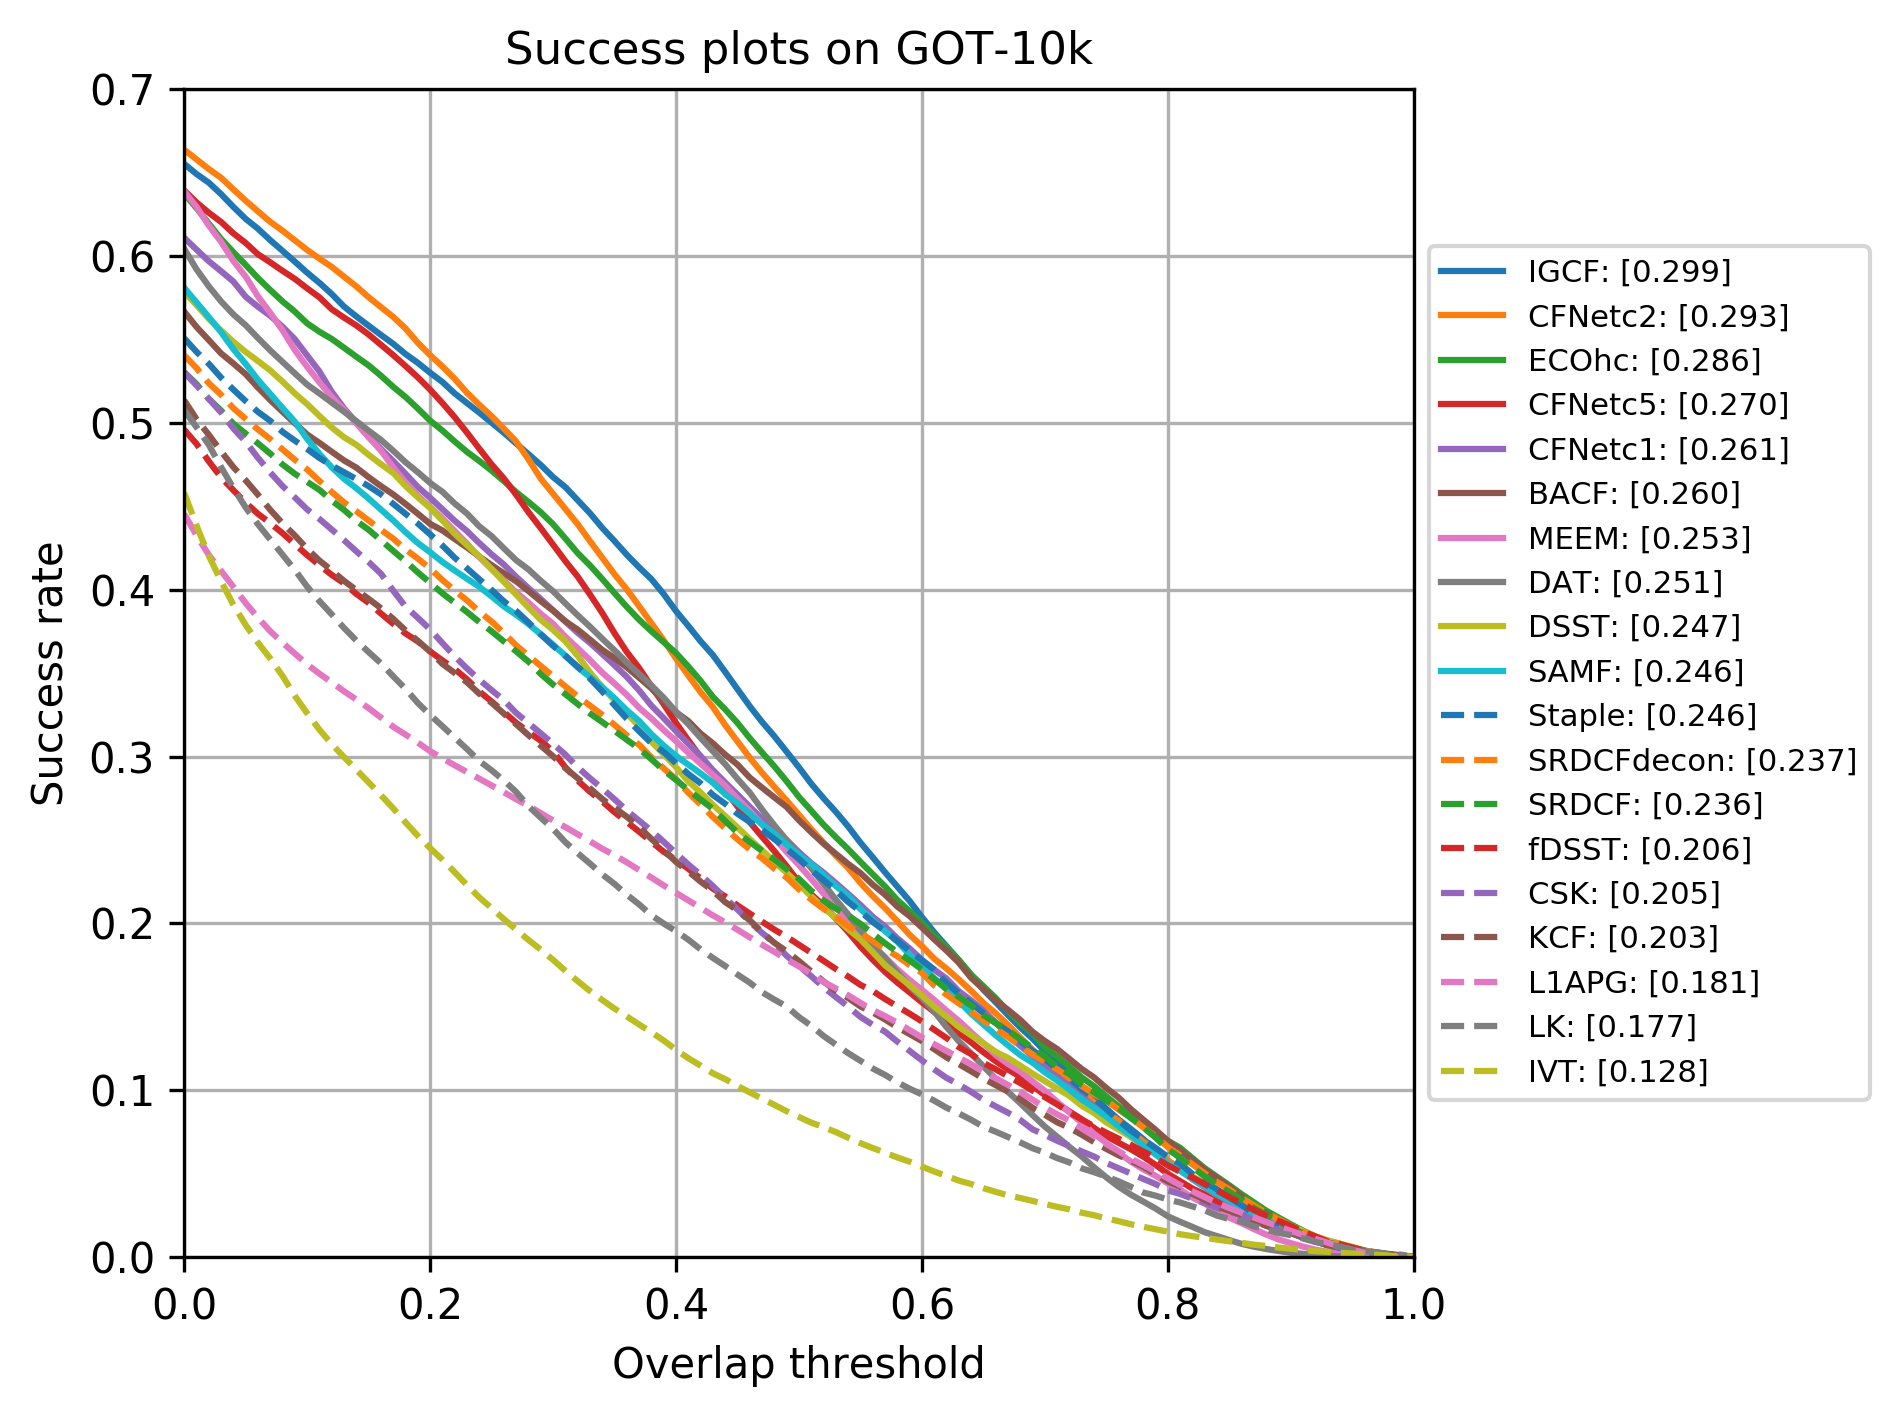
\includegraphics[width=0.8\textwidth]{Img/IGCF/got10k/success_plot.png}
    \caption{在 GOT-10k \cite{GOT-10k} 上的总体性能,按其平均重叠(AO)得分进行排名。}
    \label{fig:IGCF_got10k}
\end{figure}

\subsection{对 VOT2016 的评估}
VOT2016 \cite{Kristan2016TheVO} 数据集包含来自 VOT2015 的 60 个序列,具有改进的注释。VOT2016 的评估指标与 VOT2015 相同,即准确性、鲁棒性和 EAO。

我们将所提出的算法与以下跟踪器进行了比较:
CSRDCF \cite{Lukezic2017DiscriminativeCF},SRDCF \cite{Danelljan2015LearningSR},TGPRfSRDCF \cite{gao2018tracking},DeepSRDCF \cite{Danelljan2015ConvolutionalFF},TCNN \cite{nam2016modeling}, Staple \cite{Bertinetto2016StapleC},EBT \cite{Zhu2016BeyondLS},NSAMF \cite{Hua2015OnlineOT} 和 Struck \cite{Hare2011StruckSO}。图 \ref{fig:vot16} 显示了 VOT2016 上 EAO 的性能。与所列出的方法相比,我们的方法以 0.330 的 EAO 得分达到最佳结果。

\subsection{对 GOT-10k 的评估}
GOT-10k \cite{GOT-10k} 是近期提出的用于通用目标跟踪的数据库。该数据集具有超过 10000 个真实运动目标的视频片段和超过 150 万个手动标记的边界框,包含了现实世界中的 563 类运动目标和 87 种运动模式。
我们在 GOT-10k 测试子集上评估跟踪器,包括 180 段视频,具有 84 个目标类别和 32 个运动模式。
GOT-10k 的评估指标是平均重叠(AO),它表示所有真实边界框和估计边界框之间重叠的平均值。

我们将本文提出的 IGCF 算法与以下跟踪器进行了比较:CFNetc2 \cite{Valmadre2017EndtoEndRL},ECOhc \cite{Danelljan2017ECOEC},CFNetc5 \cite{Valmadre2017EndtoEndRL},CFNetc1 \cite{Valmadre2017EndtoEndRL}, BACF \cite{Galoogahi2017LearningBC},MEEM \cite{Zhang2014MEEMRT},DAT \cite{Possegger2015InDO},DSST \cite{Danelljan2014AccurateSE},SAMF \cite{Li2014ASA},Staple \cite{Bertinetto2016StapleC},SRDCFdecon \cite{Danelljan2016AdaptiveDO},SRDCF \cite{Danelljan2015LearningSR},fDSST \cite{Danelljan2017DiscriminativeSS},CSK \cite{Henriques2012ExploitingTC},KCF \cite{henriques2014high-speed},L1APG \cite{Bao2012RealTR},LK \cite{Shi1994GoodFT} 和 IVT \cite{Ross2007IncrementalLF}。评估的跟踪器的成功图如图 \ref{fig:got10k}所示。它代表重叠度量超过阈值的帧相对于不同阈值的百分比。
本章提出的方法在 GOT-10k 测试集上的 AO 得分为 0.299,优于所有其他列出的竞争跟踪算法。
在文献 CFNet \cite{Valmadre2017EndtoEndRL} 中,Valmadre 等人将相关滤波器表示为深度神经网络中的一个可微层,以端到端方式学习相关滤波跟踪器的特征表示。作者采用一个不对称的孪生网络,利用训练图像学习线性模板,并通过互相关在测试图像上搜索目标位置。CFNetc2 在 GOT-10k 测试集上的 AO 得分为 0.293,取得了较好的跟踪结果,说明端到端学习有利于提高跟踪性能。然而,该方法仅利用 2 层卷积网络提取图像特征,使用更多卷积层时(如 5 层)反而会导致跟踪性能下降,这限制了 CFNet 的潜力。
而本章提出的网络 InstMask 基于 ResNet 设计,具有更多卷积层,可有效提取图像的高层语义信息,因此取得了更好的跟踪性能。
\begin{figure}[t]
\centering
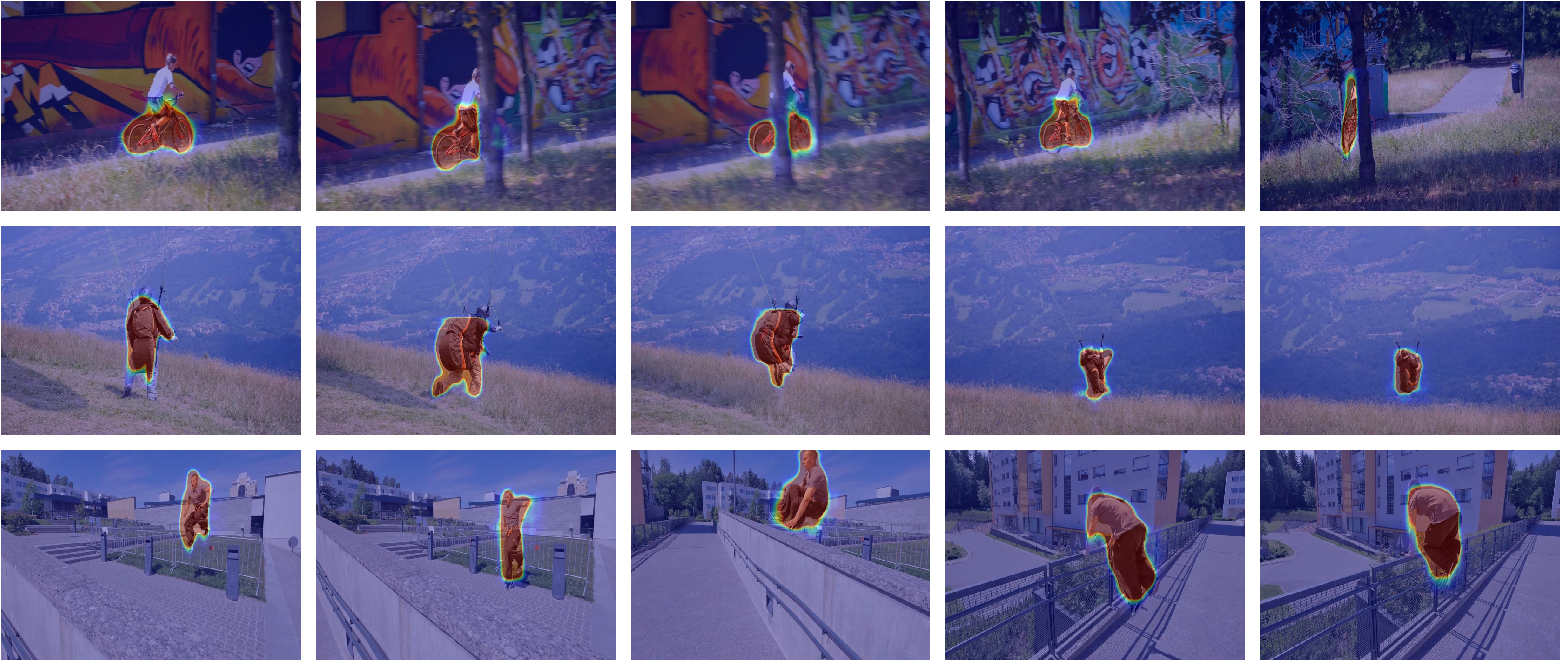
\includegraphics[width=\textwidth]{Img/IGCF/davis.pdf}
\caption{我们的方法在 DAVIS2016 VAL 数据集中的定性结果。}
\label{fig:davis}
\end{figure}

\subsection{对 DAVIS2016 的评估}
配备有 InstMask 模块的跟踪器不仅可以很好地执行目标跟踪,还可以用于视频分割。DAVIS \cite{Perazzi2016} 是一个视频目标分割数据集,它由 50 个高质量视频序列组成,包含常见的视频目标分割挑战,例如遮挡、运动模糊和表观变化等。我们在 DAVIS2016 的验证集上进行了定性实验。可视化结果如图 \ref{fig:davis} 所示。结果表明,提出的 IGCF 可以准确地恢复目标的轮廓,这在一定程度上解释了 IGCF 可以提高跟踪性能的原因。

\section{本章小结}
在本文中,我们提出了一种新颖的跟踪器,该跟踪器结合了深度神经网络和相关滤波器的优点来提高目标跟踪的性能。
InstMask 用于约束相关滤波器的学习过程。基于实例级别的分割,我们进一步提出了一种自校正机制,以减轻对相关滤波器的漂移。
通过与最新的跟踪器进行比较,实验结果显示了该方法的出色鲁棒性和效率。